\documentclass[12pt]{article}

\usepackage{sbc-template}
\usepackage{graphicx,url}
\usepackage[utf8]{inputenc}
\usepackage[brazil]{babel}
%\usepackage[latin1]{inputenc}  

     
\sloppy

\title{Classificação de Acidentes Rodoviários a Partir de Fatores de Tráfego e Pavimento no Brasil}

\author{Augusto D. N. Oliveira\inst{1}, Vitor Uchikawa\inst{2}}

\address{
    Universidade Federal de Santa Catarina (UFSC) -- Campus Joinville\\
    Programa de Pós-Graduação em Engenharia de Sistemas Eletrônicos (PPGESE)\\
    Joinville -- SC -- Brasil
    \email{augusto-\_-14@hotmail.com, vitor.uchikawa@gmail.com}
}

\begin{document}

\maketitle

\begin{abstract}
This study analyzes the relationship between road accident characteristics and severity classification in Brazil. Data from the Federal Highway Police, DNIT, and ANTT were integrated, resulting in 187,348 accident records and 13 predictor variables. A multiclass CatBoost classifier was trained with stratified data splitting, class weights, and SHAP-based interpretation. On the test set, the model achieved 77.78\% accuracy, 55.50\% balanced accuracy, and 57.21\% macro F1-score. Accident type, highway, and accident cause were the most important features according to the model. Statistical association measures and predictive importance were analyzed jointly, emphasizing that these results describe associations and predictive contributions rather than causal effects.
\end{abstract}
     
\begin{resumo} 
Este estudo analisa a relação entre as características dos acidentes rodoviários e sua classificação de severidade no Brasil. Foram integrados dados da Polícia Rodoviária Federal, do DNIT e da ANTT, resultando em 187.348 registros de acidentes e 13 variáveis preditoras. Foi treinado um classificador CatBoost multiclasse, com divisão estratificada dos dados, pesos de classe e interpretação por meio de SHAP. No conjunto de teste, o modelo alcançou 77,78\% de acurácia, 55,50\% de acurácia balanceada e 57,21\% de F1-score macro. Tipo de acidente, rodovia e causa do acidente foram as características de maior importância segundo o modelo. Medidas de associação estatística e importância preditiva foram analisadas conjuntamente, ressaltando que os resultados descrevem associações e contribuições preditivas, e não efeitos causais.
\end{resumo}

\section{Introdução}

\subsection{Contextualização}

A classificação dos acidentes rodoviários envolve características do condutor, da via, do ambiente e da própria ocorrência \cite{who2023roadsafety}. Para examinar as relações entre essas características e o desfecho registrado, é necessário reunir informações de diferentes dimensões do sistema rodoviário.

Nesse sentido, os dados abertos da Polícia Rodoviária Federal (PRF) apresentam informações sobre localização, causa, tipo de acidente, fase do dia, condições meteorológicas e características da pista \cite{prf_dados_abertos}. Esses registros, organizados em nível de ocorrência, constituíram a principal fonte de dados utilizada neste trabalho.

Embora reúna informações detalhadas sobre os acidentes, a base da PRF não contempla todos os fatores pertinentes à predição da classificação, como aspectos relacionados ao tráfego e à conservação das rodovias. Por esse motivo, ela foi complementada com o volume de veículos nas praças de pedágio, fornecido pela Agência Nacional de Transportes Terrestres (ANTT) \cite{antt_dados_abertos}, e com o Índice de Condição da Manutenção (ICM), disponibilizado pelo Departamento Nacional de Infraestrutura de Transportes (DNIT) \cite{dnit_icm}.

A partir dessa integração, foram considerados os registros de acidentes disponíveis a partir de 1º de novembro de 2023. Cada ocorrência foi associada, quando disponíveis, ao volume mensal da praça de pedágio mais próxima e ao ICM do trecho correspondente.

Após o pré-processamento, o conjunto de dados foi consolidado em 187.348 registros de acidentes com 13 variáveis preditoras. Nesse conjunto, a classificação do acidente foi definida como variável-alvo e dividida em três classes: com vítimas fatais, com vítimas feridas e sem vítimas.

Para representar as diferentes dimensões presentes na base, foram selecionadas variáveis relacionadas ao tipo e à causa do acidente, à fase do dia, à condição meteorológica, ao tipo de pista, ao traçado da via, ao trecho da rodovia, ao volume de pedágio e ao ICM. A partir dessas informações, também foram construídas variáveis para representar a presença de fator humano, a inclinação da via e sua geometria horizontal.

Com o conjunto de dados estruturado, a análise estatística foi utilizada para examinar as associações entre as variáveis selecionadas e a classificação dos acidentes. Em seguida, o algoritmo CatBoost foi empregado para realizar a classificação multiclasse e estimar a importância das variáveis, com tratamento direto dos atributos categóricos \cite{prokhorenkova2018catboost}.

\subsection{Problema de pesquisa}

A composição do conjunto de dados apresenta desafios que devem ser considerados durante a modelagem. Entre eles, está o desbalanceamento das classes, pois os acidentes com vítimas feridas representam a maior parte dos registros, enquanto os acidentes com vítimas fatais são menos frequentes.

Essa diferença na quantidade de registros favorece a classe majoritária durante o treinamento. Como consequência, o modelo pode apresentar desempenho global elevado e, ao mesmo tempo, ter dificuldade em reconhecer as classes com menor número de ocorrências.

Além do desbalanceamento, a definição das variáveis preditoras requer atenção ao vazamento do alvo. Informações disponibilizadas acerca de mortos e feridos revelariam ao modelo dados diretamente relacionados ao desfecho, comprometendo a avaliação.

Mesmo após a exclusão dessas variáveis, as relações observadas nos dados devem ser interpretadas como associações estatísticas, e não como relações de causa e efeito. Uma característica pode estar associada à classificação do acidente sem necessariamente explicar o desfecho observado.

Considerando essas limitações, o problema de pesquisa consiste em avaliar em que medida as características dos acidentes e das rodovias permitem distinguir as três classes analisadas. Também se busca identificar quais variáveis apresentam maior associação com a classificação e maior contribuição para o desempenho do modelo.

\subsection{Objetivo Geral}

Diante disso, o objetivo geral deste trabalho é analisar as relações entre as características dos acidentes rodoviários e sua classificação. Pretende-se ainda desenvolver e avaliar um modelo de aprendizado de máquina para classificar as ocorrências registradas pela PRF e identificar as variáveis de maior relevância preditiva.

\subsection{Objetivos específicos}

Os objetivos específicos são: (i) integrar e padronizar os dados da PRF, da ANTT e do DNIT; (ii) associar cada acidente ao volume mensal da praça de pedágio mais próxima e ao ICM do trecho; (iii) examinar a qualidade, a distribuição e os valores ausentes dos dados; (iv) selecionar e construir variáveis preditoras, evitando vazamento do alvo; (v) medir associações por V de Cramér, intervalo de Wilson, Kruskal--Wallis, epsilon ao quadrado e correlação de Spearman; (vi) treinar e ajustar um classificador CatBoost considerando o desbalanceamento; e (vii) avaliar o modelo e identificar as variáveis mais importantes.

\section{Fundamentação teórica}

A análise de dados compreende desde a caracterização inicial das informações até a construção de modelos capazes de identificar padrões ou realizar predições. Para fundamentar essa análise, esta seção do trabalho abordará a análise exploratória dos dados, os métodos utilizados para investigar associações entre variáveis, o algoritmo de classificação empregado e as métricas adotadas para avaliar seu desempenho.

\subsection{Análise exploratória de dados}

A análise exploratória de dados consiste na avaliação preliminar do conjunto de dados com o objetivo de compreender suas principais características, identificar padrões e detectar outliers \cite{tukey1977eda}. Nessa etapa, busca-se descrever os dados sem estabelecer inicialmente um modelo específico para explicar seu comportamento, utilizando principalmente representações gráficas e medidas descritivas.

A forma de exploração depende da natureza da variável analisada. Para variáveis quantitativas, histogramas podem ser utilizados para observar a distribuição dos valores, enquanto diagramas de dispersão permitem examinar visualmente a relação entre pares de variáveis. Quando diversas variáveis quantitativas são consideradas, matrizes de diagramas de dispersão permitem visualizar conjuntamente suas relações par a par \cite{james2023islp}.

Nas análises que envolvem uma variável quantitativa e uma variável categórica, diagramas de caixa (boxplots) permitem comparar a distribuição da variável quantitativa entre diferentes grupos. Esse tipo de representação permite visualizar diferenças na distribuição dos valores entre as categorias, propiciando uma análise inicial das possíveis distinções entre os grupos \cite{james2023islp}.

Essas representações gráficas geralmente são complementadas por estatísticas descritivas que resumem numericamente as principais características das variáveis. Em conjunto, esses recursos servem para a compreensão inicial dos dados a serem investigados posteriormente por meio de medidas de associação e testes estatísticos \cite{james2023islp}.

\subsection{Análise estatística de associação e métricas utilizadas}

A análise estatística permite examinar as relações e suas intensidades entre variáveis. A escolha do método estatístico depende do tipo de variável considerada e do objetivo da análise.

Neste trabalho, o $V$ de Cramér é utilizado para avaliar associações entre variáveis categóricas; o teste de Kruskal--Wallis e o $\epsilon^2$ são empregados na comparação de variáveis numéricas entre grupos; o intervalo de Wilson é utilizado na estimação de proporções; e a correlação de Spearman é aplicada à análise de associações monotônicas entre variáveis numéricas. Esses métodos são apresentados nas subseções a seguir.

Na análise realizada, esses métodos foram aplicados para avaliar associações entre os fatores selecionados e a severidade dos acidentes. Os resultados são posteriormente comparados à importância das variáveis no modelo de classificação, permitindo discutir de forma complementar as associações estatísticas e as contribuições preditivas \cite{agresti2007,kruskal1952,brown2001interval,spearman1904}.

\subsubsection{$V$ de Cramér}

A associação entre duas variáveis categóricas pode ser analisada por meio de uma tabela de contingência. Sob a hipótese de independência, a frequência esperada para a célula $(i,j)$ é dada por \cite{agresti2007}

\begin{equation}
    \hat{\mu}_{ij} = \frac{n_{i+}n_{+j}}{n},
\end{equation}
em que $n_{i+}$ e $n_{+j}$ são os totais da linha e da coluna, respectivamente, e $n$ é o número total de observações. A estatística qui-quadrado de Pearson compara as frequências observadas e esperadas \cite{agresti2007}:

\begin{equation}
    \chi^2 = \sum_{i=1}^{r}\sum_{j=1}^{c}\frac{(n_{ij}-\hat{\mu}_{ij})^2}{\hat{\mu}_{ij}}.
\end{equation}
Embora o teste qui-quadrado permita verificar a existência de evidências de associação, ele não indica diretamente sua intensidade \cite{agresti2007}. Para isso, pode-se utilizar o $V$ de Cramér, definido por \cite{navarro2015learning}

\begin{equation}
    V = \sqrt{\frac{\chi^2}{n(k-1)}},
    \qquad
    k = \min(r,c),
\end{equation}
onde $r$ e $c$ correspondem ao número de linhas e colunas da tabela. O coeficiente pode variar entre $0$ e $1$, de modo que valores próximos de $0$ indicam uma associação fraca ou inexistente, enquanto valores próximos de $1$ indicam uma associação forte \cite{navarro2015learning}.

\subsubsection{Kruskal--Wallis}

O teste de Kruskal--Wallis é um método não paramétrico utilizado para comparar uma variável quantitativa entre vários grupos independentes, sendo uma alternativa à ANOVA  quando seus pressupostos não puderem ser atendidos \cite{field2009discovering}. O procedimento baseia-se na ordenação conjunta das observações, independentemente do grupo ao qual pertencem, atribuindo-lhes postos em ordem crescente. Em seguida, os postos são novamente separados segundo os grupos e utilizados no cálculo da estatística do teste.

A estatística $H$ é obtida a partir das somas dos postos de cada grupo e pode ser expressa por

\begin{equation}
H =
\frac{12}{N(N+1)}
\sum_{i=1}^{k}
\frac{R_i^2}{n_i}
- 3(N+1),
\end{equation}
em que $R_i$ representa a soma dos postos do $i$-ésimo grupo, $n_i$ corresponde ao número de observações desse grupo, $N$ é o número total de observações e $k$ é o número de grupos \cite{field2009discovering}. Sob a hipótese nula de ausência de diferenças entre os grupos, a estatística $H$ é avaliada por meio de uma distribuição qui-quadrado com $k-1$ graus de liberdade.

Um resultado estatisticamente significativo indica que existe diferença entre pelo menos dois dos grupos analisados, mas não identifica quais grupos diferem entre si. Quando essa identificação é necessária, devem ser realizadas comparações posteriores apropriadas, com controle do erro associado às múltiplas comparações \cite{field2009discovering}.

\subsubsection{Epsilon²}

O epsilon-quadrado ($E_R^2$) é uma medida de tamanho de efeito que pode ser aplicada em conjunto com o teste de Kruskal--Wallis. Enquanto o teste busca evidências de diferenças entre os grupos, o valor de $p$ resultante não informa diretamente a magnitude dessas diferenças. Nesse sentido, o uso de uma medida de tamanho de efeito complementa a análise ao fornecer uma indicação da intensidade da relação observada \cite{tomczak2014need}. Para o teste de Kruskal--Wallis, o epsilon-quadrado pode ser calculado por \cite{tomczak2014need}:

\begin{equation}
E_R^2 = \frac{H}{(n^2-1)/(n+1)},
\end{equation}
em que $H$ representa a estatística do teste de Kruskal--Wallis e $n$ o número total de observações. O coeficiente varia de 0 a 1, sendo que valores próximos ao limite inferior indicam pouca relação, enquanto valores próximos ao limite superior indicam uma relação mais acentuada \cite{tomczak2014need}.

\subsubsection{Intervalo de Wilson}

O intervalo de Wilson é utilizado para estimar um intervalo de confiança para uma proporção binomial. Esse método é baseado no teste de escore e apresenta propriedades de cobertura mais adequadas que o intervalo de Wald, especialmente em amostras pequenas ou quando a proporção está próxima de 0 ou 1 \cite{brown2001interval}.

Na aplicação do intervalo de Wilson, inicialmente contabiliza-se o número $X$ de ocorrências de interesse em um total de $n$ observações, obtendo-se a proporção amostral $\hat{p}=X/n$. Em seguida, define-se o nível de confiança e o valor crítico correspondente da distribuição normal padrão, como $z=1{,}96$ para um intervalo de 95\%. Os limites inferior e superior são então obtidos pelos valores da proporção populacional que não seriam rejeitados pelo teste de escore nesse nível de significância \cite{agresti2007}. Dessa forma, determina-se uma faixa de valores plausíveis para a proporção populacional.

\subsubsection{Correlação de Spearman}

O coeficiente de correlação de Spearman ($r_s$) é uma medida não paramétrica utilizada para avaliar a associação entre duas variáveis. Enquanto a correlação de Pearson se concentra em relações lineares, a correlação de Spearman considera relações monotônicas, nas quais as variáveis tendem a crescer ou decrescer de forma consistente \cite{navarro2015learning}. Como não exige os mesmos pressupostos paramétricos da correlação de Pearson, pode ser aplicado a dados que não seguem uma distribuição normal e a variáveis em escala ordinal \cite{field2009discovering}.

Seu cálculo é baseado na ordenação das observações em postos. Inicialmente, os valores de cada variável são substituídos por suas respectivas posições na ordenação e, em seguida, aplica-se o cálculo da correlação de Pearson sobre esses postos \cite{field2009discovering}. Na ausência de empates entre os postos, uma forma usual de expressar o coeficiente é \cite{kim2018statistical}:

\begin{equation}
r_s = 1 - \frac{6\sum_{i=1}^{n}d_i^2}{n(n^2-1)},
\end{equation}
em que $d_i$ representa a diferença entre os postos das duas variáveis para a $i$-ésima observação e $n$ corresponde ao número de observações. O coeficiente varia de $-1$ a $1$, sendo que o sinal indica a direção da associação e sua magnitude indica a intensidade da relação \cite{kim2018statistical}. A significância estatística da associação pode ser avaliada pelo valor de $p$, permitindo verificar se há evidências de uma relação entre as variáveis analisadas \cite{field2009discovering}.

\subsection{CatBoost}

No aprendizado supervisionado, as observações são anotadas com o alvo de predição. A partir desses dados, procura-se estimar uma função capaz de relacionar as entradas à resposta, com o objetivo de realizar predições para observações inéditas. Quando a variável resposta assume valores categóricos, como diferentes classes de gravidade de um acidente, caracteriza-se um problema de classificação \cite{james2023islp}.

Entre os métodos supervisionados, os métodos de conjunto combinam modelos simples para obter um preditor mais robusto. O boosting segue essa abordagem ao construir os modelos sequencialmente, de modo que cada novo modelo utiliza informações dos anteriores para corrigir os erros que ainda persistem. Quando árvores de decisão são utilizadas como modelos-base, árvores de menor porte são adicionadas gradualmente ao conjunto. Parâmetros como o número de árvores, a profundidade e a taxa de aprendizado controlam a complexidade e a velocidade do ajuste \cite{james2023islp}.

O gradient boosting toma esse processo sequencial de base e passa a orientá-lo pela otimização iterativa da função de perda. Em cada iteração, uma nova árvore é ajustada para aproximar o gradiente negativo da perda associada ao modelo atual, buscando reduzir os erros remanescentes. A atualização do modelo pode ser representada por \cite{prokhorenkova2018catboost}:

\begin{equation}
F_t(x) = F_{t-1}(x) + \alpha h_t(x),
\end{equation}
em que $F_t(x)$ é o modelo após a iteração $t$, $F_{t-1}(x)$ representa o modelo anterior, $h_t(x)$ é o novo preditor-base e $\alpha$ corresponde à taxa de aprendizado que controla a contribuição desse preditor.

O CatBoost (Categorical Boosting) é uma implementação do gradient boosting desenvolvida para lidar com variáveis categóricas. Uma abordagem convencional consiste em transformar cada categoria em variáveis binárias por meio de one-hot encoding, o que pode gerar um número elevado de variáveis quando existem categorias com alta cardinalidade. Outra possibilidade é substituir as categorias por estatísticas calculadas a partir da variável resposta. Entretanto, quando o valor da própria observação participa desse cálculo, ocorre vazamento da informação do alvo, o que pode produzir diferenças entre o comportamento do modelo nos dados de treinamento e em novas observações \cite{prokhorenkova2018catboost}.

Para lidar com esse problema, o CatBoost utiliza estatísticas ordenadas para representar as variáveis categóricas. Durante o treinamento, os dados são organizados em diferentes ordens aleatórias e, para cada observação, a estatística de sua categoria é calculada apenas com base nas observações anteriores. O mesmo princípio é aplicado no ordered boosting: ao calcular o gradiente de uma observação, o algoritmo utiliza um modelo treinado somente com os dados que aparecem antes dela, sem incluir informações sobre sua classe. Essa estratégia ajuda a reduzir o vazamento da variável resposta e as diferenças entre as predições realizadas nos dados de treinamento e teste. O CatBoost também utiliza árvores de decisão simétricas, nas quais o mesmo critério de divisão é aplicado a todos os nós de um mesmo nível, formando estruturas balanceadas e eficientes \cite{prokhorenkova2018catboost}.

\subsection{Métricas de avaliação}

A avaliação de modelos deve considerar não apenas a proporção total de previsões corretas, mas também o desempenho obtido em cada classe. Essa distinção é importante quando existe desbalanceamento entre as classes, pois uma elevada taxa global de acertos pode ocultar um desempenho insatisfatório nas classes menos frequentes \cite{james2023islp}. Neste trabalho, são utilizadas a acurácia, a acurácia balanceada, a precisão, a revocação, o F1-score e a matriz de confusão.

A primeira métrica observada foi a acurácia, que corresponde à proporção de observações classificadas corretamente em relação ao total. Embora seja simples e forneça um panorama geral do desempenho, ela pode atribuir maior peso às classes mais frequentes \cite{james2023islp,sklearn_metrics}. Para complementar essa avaliação, utiliza-se a acurácia balanceada, definida pela média da revocação obtida em cada classe. Dessa forma, cada classe contribui igualmente para o resultado, independentemente de sua frequência \cite{sklearn_metrics}.

A precisão, por sua vez, mede a proporção de previsões atribuídas a uma determinada classe que estão corretas, enquanto a revocação representa a proporção das observações realmente pertencentes à classe que foram corretamente identificadas. O F1-score combina essas duas medidas por meio de sua média harmônica, produzindo uma única métrica que considera simultaneamente precisão e revocação \cite{sklearn_metrics}.

Em problemas multiclasse, essas métricas podem ser calculadas individualmente para cada classe e posteriormente agregadas. Nesse sentido, o F1 macro corresponde à média simples dos valores de F1 das classes, enquanto o F1 ponderado considera a quantidade de observações de cada classe como peso \cite{sklearn_metrics}. F1 macro é utilizado neste trabalho como métrica guia para a seleção do modelo, pois permite avaliar o desempenho nas diferentes classes sem favorecer aquelas com maior número de observações.

Por fim, a matriz de confusão complementa essas métricas ao apresentar, em forma de tabela, a relação entre as classes reais e as previstas pelo modelo. Os valores da diagonal representam as classificações corretas, enquanto os demais indicam os erros de classificação. Dessa forma, sua análise também permite identificar quais classes são mais frequentemente confundidas entre si \cite{james2023islp}.

\subsection{Fatores Associados aos Acidentes Rodoviários}
A severidade dos acidentes rodoviários é um fenômeno multifatorial, associado à interação entre comportamento humano, características da via, condições ambientais e tráfego. Estudos realizados no Brasil destacam a relação entre segurança viária e características de pavimento, geometria, sinalização e condições da via \cite{carmo2019,costa2022}. Neste estudo, esses fatores são representados por causas e tipo de acidente, condições meteorológicas, geometria e tipo de pista, rodovia, quilômetro, condição do pavimento e volume de tráfego. A variável \textit{fator\_humano} explicita a dimensão comportamental a partir das causas registradas.

A severidade é classificada em três categorias: acidentes sem vítimas, com vítimas feridas e com vítimas fatais. A condição da rodovia também pode estar relacionada a aspectos operacionais, como consumo de combustível, tempo de viagem e custos de manutenção, além de impactos ambientais \cite{bartholomeu2008}. Neste trabalho, essas características são tratadas como fatores associados e utilizadas para investigar padrões preditivos, sem interpretação causal.

\subsection{Trabalhos Relacionados}
Estudos sobre severidade de acidentes combinam métodos estatísticos e aprendizado de máquina para identificar fatores associados e melhorar a capacidade de classificação.

Carmo e Raia Junior \cite{carmo2019} analisaram rodovias federais em áreas urbanas da região Sul do Brasil, integrando registros da PRF a informações de pavimento, geometria e sinalização. Costa Júnior e Santos Júnior \cite{costa2022} utilizaram dados da PRF de 2017 a 2019 e regressão logística para investigar o risco de morte em rodovias federais brasileiras. Esses trabalhos evidenciam a relevância de características da infraestrutura, localização e condições de operação para a análise da segurança viária.

No campo do aprendizado de máquina, Samerei, Aghabayk e Montella \cite{samerei2024} compararam métodos de ensemble para classificação de severidade e obtiveram o melhor desempenho com CatBoost, utilizando SHAP para interpretação. Xie et al. \cite{xie2025} também combinaram CatBoost e SHAP em um framework interpretável para previsão de acidentes fatais. Esses trabalhos fornecem suporte metodológico para a utilização conjunta de CatBoost e técnicas de explicabilidade.

Este estudo diferencia-se por integrar dados da PRF, DNIT e ANTT e combinar classificação multiclasse, análise estatística e explicabilidade, com foco em fatores de tráfego, pavimento, infraestrutura e comportamento humano no contexto brasileiro.

\section{Materiais e Métodos}
\subsection{Pré-processamento}
As bases de dados brutas da PRF, DNIT e ANTT passaram por pré-processamento, incluindo padronização de formatos, correção de inconsistências e remoção de registros duplicados ou incompletos. As variáveis categóricas foram mantidas como categóricas e as numéricas em formato numérico. A variável km foi mantida no conjunto final e utilizada tanto na integração espacial quanto como característica preditiva. Por sua natureza espacial, sua contribuição deve ser interpretada com cautela, pois pode capturar padrões associados à localização dos acidentes. As variáveis volume\_pedagio e icm, que apresentam valores ausentes, foram preservadas no conjunto de dados, com seu tratamento realizado no pipeline de modelagem.

\subsection{Integração das Bases}
A integração das informações provenientes da PRF, DNIT e ANTT foi realizada utilizando o método de Localização de Referência Linear. A associação foi feita utilizando a Unidade Federativa (UF), a rodovia (BR), o quilômetro (KM) e o sentido de tráfego como chaves de referência. Essa abordagem possibilitou a vinculação de cada ocorrência de acidente a características do trecho rodoviário onde ocorreu, incluindo dados de pavimento e tráfego, criando um dataset unificado.

\subsection{Engenharia de Características (Feature Engineering)}
Com base nos dados integrados, foram criadas características para alimentar o modelo. As variáveis categóricas foram dia\_semana, br, causa\_acidente, tipo\_acidente, fase\_dia, condicao\_meteorologica, tipo\_pista, inclinacao e reta. As variáveis numéricas foram km, volume\_pedagio, icm e fator\_humano.

O fator\_humano foi construído como variável binária, derivada de causas classificadas como comportamentais ou falhas humanas. Embora exista sobreposição conceitual com causa\_acidente, ambas foram mantidas por desempenharem papéis analíticos distintos: causa\_acidente preserva a informação categórica detalhada, enquanto fator\_humano explicita uma dimensão binária de interesse e favorece a interpretação por SHAP. Variáveis irrelevantes ou que poderiam causar vazamento do alvo foram removidas.

\subsection{Modelagem e Treinamento do CatBoost}
\subsubsection{Divisão dos Dados}
O conjunto final, com 187.348 registros, foi dividido de forma estratificada em 80\% para treinamento, 10\% para validação e 10\% para teste, utilizando seed fixa em 42 para garantir a reprodutibilidade dos experimentos.

\subsubsection{Tratamento do Desbalanceamento}
A distribuição das classes foi considerada no treinamento por meio de pesos de classe, atribuindo maior peso às classes minoritárias. Os pesos utilizados foram 1,0000 para acidentes com vítimas feridas, 2,2195 para acidentes sem vítimas e 3,2952 para acidentes com vítimas fatais.

\subsubsection{Treinamento do CatBoost}
O CatBoost foi selecionado para a classificação multiclasse por lidar nativamente com variáveis categóricas e apresentar resultados favoráveis em estudos de severidade de acidentes \cite{prokhorenkova2018catboost,samerei2024,xie2025}. O treinamento utilizou pesos de classe e early stopping monitorado no conjunto de validação.

\subsubsection{Otimização de Hiperparâmetros}
Foram avaliadas 8 combinações de hiperparâmetros, variando profundidade, taxa de aprendizado e expoente dos pesos de classe. A configuração com maior F1-macro na validação foi selecionada: profundidade 8, taxa de aprendizado 0,06, expoente dos pesos 0,5, $L2$ leaf regularization igual a 8, random strength igual a 1, bagging temperature igual a 0 e 418 iterações, com F1-macro de validação igual a 0,5743.

\subsubsection{Avaliação do Modelo}
O desempenho foi avaliado no conjunto de teste por acurácia, balanced accuracy, precisão, recall, F1-score macro, métricas por classe e matriz de confusão. A explicabilidade foi analisada por SHAP, considerando a média dos valores absolutos das contribuições entre as classes \cite{lundberg2017}. Para os gráficos, valores ausentes de icm e volume\_pedagio foram excluídos apenas da cópia destinada à visualização, mantendo-se os dados originais no treinamento e na avaliação.

\section{Resultados e Discussão}
\subsection{Desempenho do CatBoost}
O conjunto final possui 187.348 registros. A distribuição das classes e as métricas gerais obtidas no conjunto de teste são apresentadas na Tabela~\ref{tab:metricas-gerais}.

\begin{table}[ht]
\centering
\caption{Distribuição das classes e métricas gerais no conjunto de teste.}
\label{tab:metricas-gerais}
\begin{tabular}{lrr}
\hline
\textbf{Medida} & \textbf{Valor absoluto} & \textbf{Percentual/valor} \\
\hline
Acidentes sem vítimas & 29.365 & 15,67\% \\
Acidentes com vítimas feridas & 144.660 & 77,21\% \\
Acidentes com vítimas fatais & 13.323 & 7,11\% \\
\hline
Acurácia & -- & 77,78\% \\
Acurácia balanceada & -- & 55,50\% \\
F1-score macro & -- & 57,21\% \\
\hline
\end{tabular}
\end{table}

As métricas de desempenho por classe são apresentadas na Tabela~\ref{tab:metricas-classes}. O melhor desempenho ocorreu na classe com vítimas feridas, enquanto as classes com vítimas fatais e sem vítimas apresentaram maior dificuldade para classificar. A diferença entre acurácia e acurácia balanceada evidencia o efeito do desbalanceamento sobre a avaliação global.

\begin{table}[ht]
\centering
\caption{Desempenho do CatBoost por classe no conjunto de teste.}
\label{tab:metricas-classes}
\begin{tabular}{lrrrr}
\hline
\textbf{Classe} & \textbf{Suporte} & \textbf{Precisão} & \textbf{Recall} & \textbf{F1-score} \\
\hline
Sem vítimas & 2.936 & 54,95\% & 35,18\% & 42,90\% \\
Com vítimas feridas & 14.466 & 83,43\% & 89,77\% & 86,48\% \\
Com vítimas fatais & 1.333 & 42,98\% & 41,56\% & 42,26\% \\
\hline
\end{tabular}
\end{table}

\subsection{Matriz de Confusão}
A matriz de confusão, com linhas representando as classes reais e colunas as classes preditas, é apresentada na Figura~\ref{fig:matriz-confusao}.

\begin{figure}[ht]
\centering
\IfFileExists{confusion_matrix.png}{%
    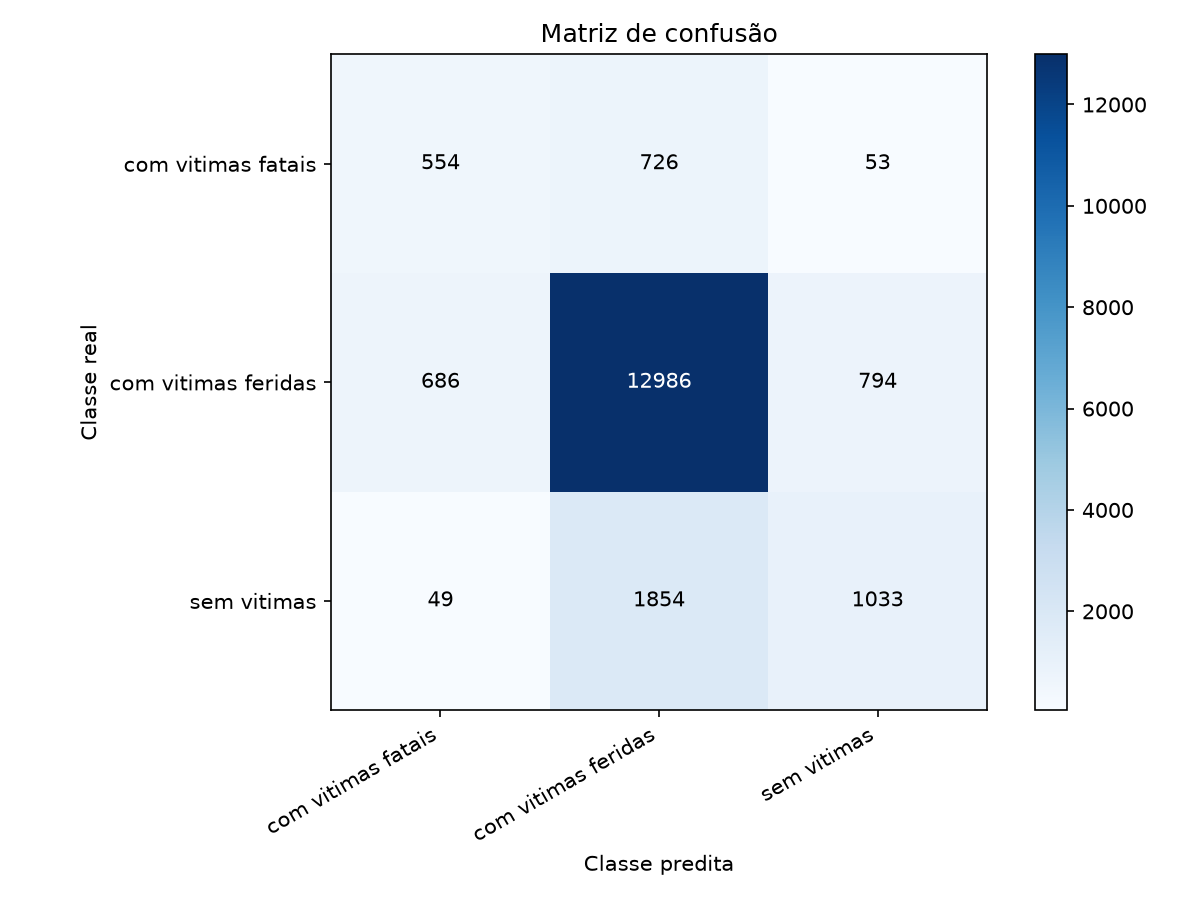
\includegraphics[width=0.85\linewidth]{confusion_matrix.png}%
}{%
    \fbox{\parbox{0.85\linewidth}{\centering\vspace{1.5cm}Placeholder: matriz de confusão\vspace{1.5cm}}}%
}
\caption{Matriz de confusão do CatBoost no conjunto de teste.}
\label{fig:matriz-confusao}
\end{figure}
O maior número de acertos ocorreu na classe com vítimas feridas, com 12.986 ocorrências. As principais confusões envolveram vítimas fatais classificadas como feridas (726 casos), vítimas feridas classificadas como fatais (686 casos) e acidentes sem vítimas classificados como feridos (1.854 casos), indicando maior confusão entre classes de severidade adjacentes.

\subsection{Importância das Características}
A importância global das características segundo o CatBoost e os valores médios absolutos de SHAP são apresentados conjuntamente na Tabela~\ref{tab:importancia-shap}.

As três características mais importantes — tipo\_acidente, br e causa\_acidente — concentraram conjuntamente aproximadamente 57,83\% da importância global. Fase\_dia, tipo\_pista e inclinacao também apresentaram contribuições relevantes. Entre as variáveis de exposição e infraestrutura, volume\_pedagio, km e icm responderam por 4,26\%, 3,61\% e 2,87\%, respectivamente, enquanto fator\_humano apresentou 1,03\%. Esses valores expressam importância preditiva global; isoladamente, não indicam a direção do efeito nem permitem estabelecer causalidade.

A análise SHAP complementa essa medida ao mostrar a direção e a magnitude das contribuições para cada classe. A Tabela~\ref{tab:importancia-shap} apresenta a média dos valores absolutos de SHAP por classe, e a Figura~\ref{fig:shap-summary-fatal} apresenta o Summary Plot para acidentes com vítimas fatais. Valores positivos favorecem a classe analisada, enquanto valores negativos atuam em sentido oposto; para variáveis numéricas e binárias, valores altos aparecem em vermelho e baixos em azul.

\begin{table}[ht]
\centering
\scriptsize
\caption{Importância global segundo o CatBoost e média dos valores absolutos de SHAP por classe.}
\label{tab:importancia-shap}
\begin{tabular}{lrrrrr}
\hline
\textbf{Característica} & \textbf{CatBoost (\%)} & \textbf{SHAP global} & \textbf{Feridas} & \textbf{Sem vítimas} & \textbf{Fatais} \\
\hline
tipo\_acidente & 26,93 & 0,2018 & 0,1251 & 0,2792 & 0,2010 \\
br & 16,01 & 0,1461 & 0,1582 & 0,0876 & 0,1926 \\
causa\_acidente & 14,90 & 0,1297 & 0,0919 & 0,1538 & 0,1432 \\
fase\_dia & 7,84 & 0,0956 & 0,1123 & 0,0531 & 0,1214 \\
tipo\_pista & 6,91 & 0,0391 & 0,0295 & 0,0441 & 0,0439 \\
inclinacao & 5,41 & 0,0546 & 0,0291 & 0,0596 & 0,0751 \\
dia\_semana & 5,08 & 0,0354 & 0,0357 & 0,0465 & 0,0239 \\
volume\_pedagio & 4,26 & 0,0329 & 0,0418 & 0,0263 & 0,0307 \\
condicao\_meteorologica & 4,22 & 0,0292 & 0,0165 & 0,0342 & 0,0367 \\
km & 3,61 & 0,0114 & 0,0096 & 0,0120 & 0,0126 \\
icm & 2,87 & 0,0182 & 0,0215 & 0,0206 & 0,0125 \\
fator\_humano & 1,03 & 0,0118 & 0,0145 & 0,0049 & 0,0159 \\
reta & 0,93 & 0,0102 & 0,0044 & 0,0132 & 0,0130 \\
\hline
\end{tabular}
\end{table}

Para volume\_pedagio, valores altos apresentaram contribuições predominantemente negativas na classe fatal e positivas na classe ferida, enquanto permaneceram próximos do centro na classe sem vítimas. Para fator\_humano, o valor 1 contribuiu positivamente na classe fatal, negativamente na classe ferida e próximo de zero na classe sem vítimas; sua magnitude global foi baixa (0,0118). Para icm, valores maiores, que representam pior condição do pavimento, contribuíram negativamente nas classes fatal e ferida e apresentaram tendência positiva na classe sem vítimas. Cerca de 41\% das observações possuíam icm ausente; a filtragem ocorreu apenas na cópia destinada aos gráficos SHAP, sem alterar treinamento ou avaliação.

Entre as características geométricas, inclinacao apresentou a maior magnitude média absoluta na classe fatal (0,0751), tipo\_pista teve magnitudes próximas nas classes sem vítimas e fatais e reta apresentou contribuição discreta. Km apresentou contribuição preditiva mensurável, mas pode capturar heterogeneidade espacial dos trechos, não devendo ser interpretado como efeito causal. Os Summary Plots não demonstram, isoladamente, interações entre características; essa hipótese requer análises específicas.

\begin{figure}[ht]
\centering
\IfFileExists{shap_summary_com_vitimas_fatais.png}{%
    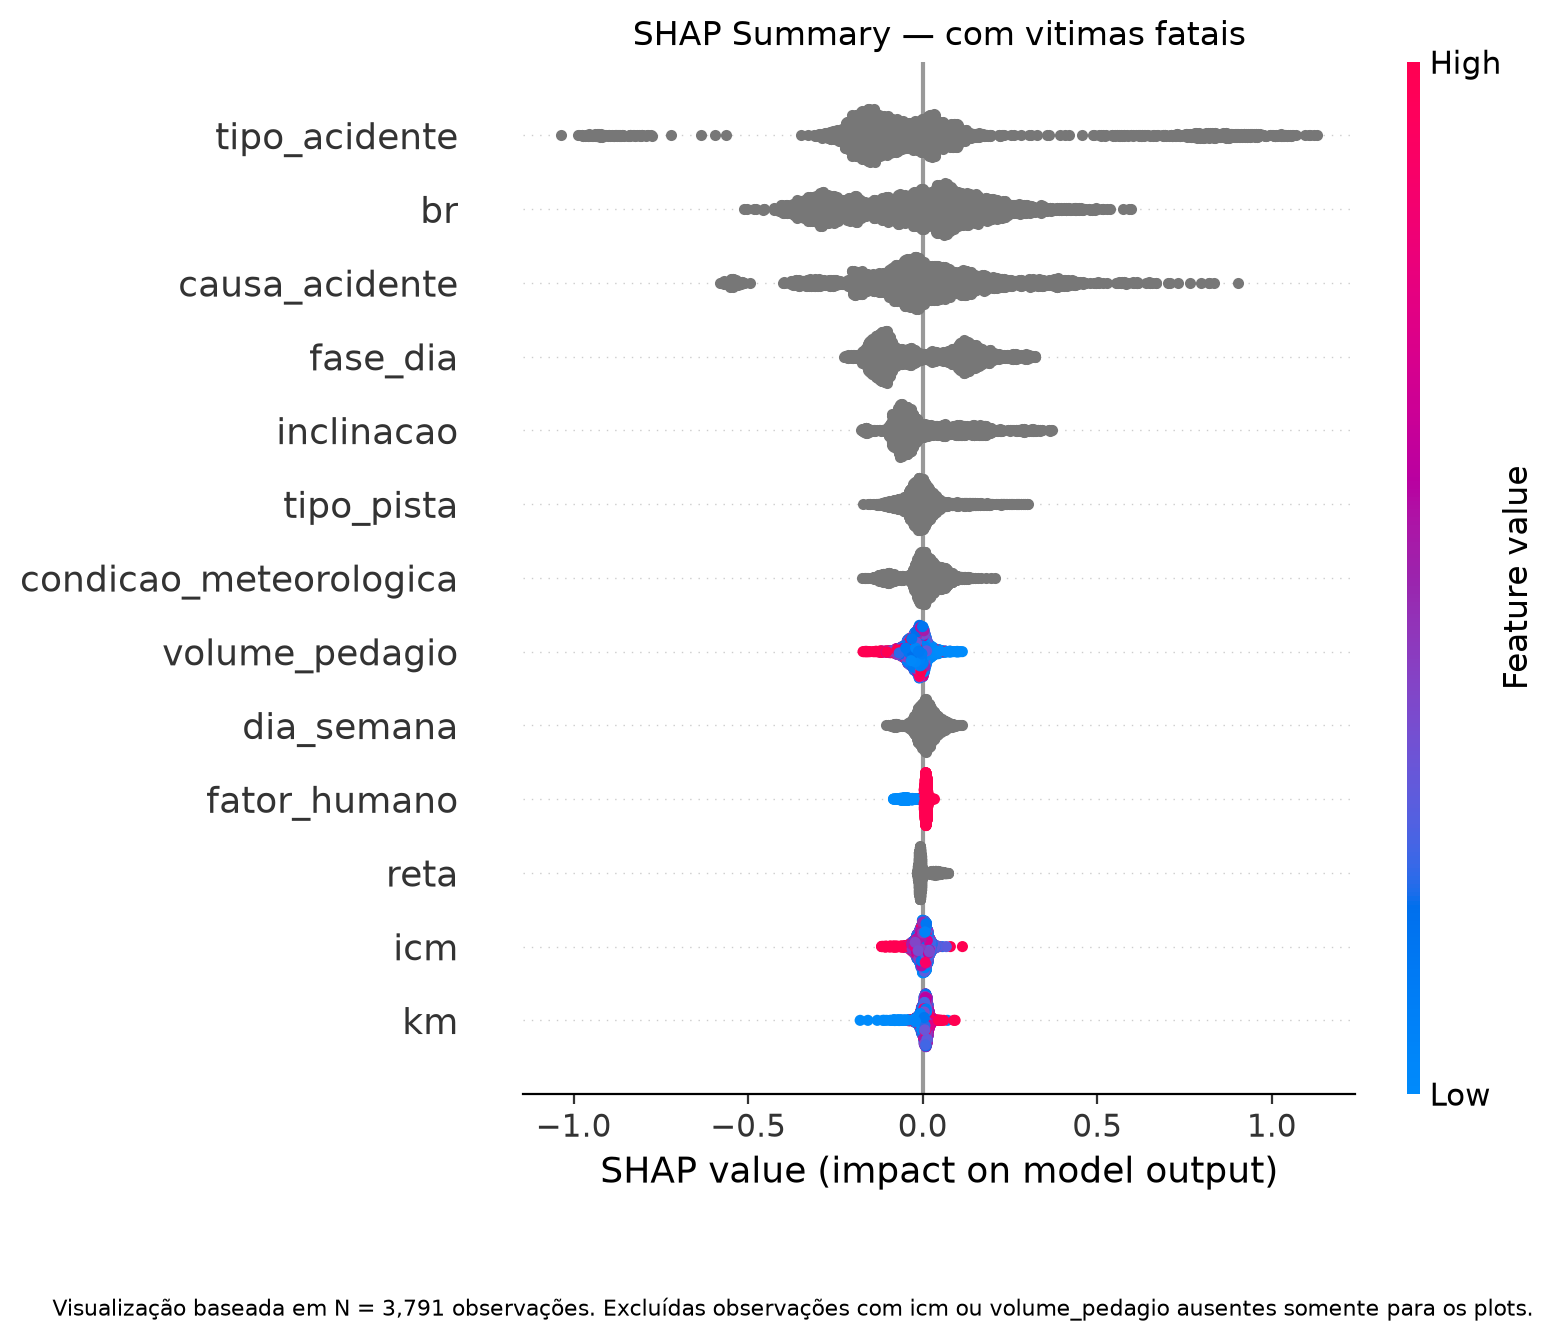
\includegraphics[width=\linewidth]{shap_summary_com_vitimas_fatais.png}%
}{%
    \fbox{\parbox{0.9\linewidth}{\centering\vspace{1.5cm}Placeholder: SHAP Summary Plot para vítimas fatais\vspace{1.5cm}}}%
}
\caption{SHAP Summary Plot para a classe com vítimas fatais.}
\label{fig:shap-summary-fatal}
\end{figure}

\subsection{Comparação entre Análise Estatística e Importância do Modelo}
A comparação entre associação estatística e importância preditiva mostra convergência para algumas variáveis. tipo\_acidente, br e causa\_acidente apresentaram simultaneamente os maiores valores de V de Cramér e as maiores importâncias no CatBoost. O V de Cramér e o $\epsilon^2$ medem intensidade de associação em análises estatísticas, enquanto a importância do modelo reflete contribuição para a predição no contexto conjunto das demais características.

Essa diferença é ilustrada por volume\_pedagio, que apresentou $\epsilon^2=0,0035$ e importância de 4,26\%; por km, com $\epsilon^2=0,0008$ e importância de 3,61\%; e por icm, com $\epsilon^2=0,0002$ e importância de 2,87\%. Para fator\_humano, o V de Cramér foi 0,1109, enquanto sua importância global no CatBoost foi 1,03\%. Os resultados mostram que associação bivariada e importância preditiva respondem a perguntas distintas e complementares.

\subsection{Limitações}
As principais limitações envolvem a heterogeneidade e possíveis inconsistências entre as bases PRF, DNIT e ANTT, além da presença de aproximadamente 41\% de valores ausentes em volume\_pedagio e icm. A definição de fator\_humano depende da classificação das causas registradas. A variável km pode capturar heterogeneidade espacial, e dependências espaciais ou temporais podem afetar a generalização; validações adicionais devem controlar essas dependências. As análises estatísticas e SHAP descrevem associações e contribuições preditivas, não causalidade. A aplicação do modelo a outros contextos requer revalidação e, se necessário, recalibração.

\section{Conclusão}
\subsection{Principais Resultados}
O CatBoost classificou a severidade dos acidentes em três classes, alcançando 77,78\% de acurácia, 55,50\% de balanced accuracy e 57,21\% de F1-score macro. O melhor desempenho ocorreu para acidentes com vítimas feridas (F1=86,48\%), enquanto as classes fatal e sem vítimas apresentaram F1 de 42,26\% e 42,90\%, respectivamente. tipo\_acidente, br e causa\_acidente foram as características de maior importância global, e a comparação com as análises estatísticas mostrou que associação marginal e contribuição preditiva não são equivalentes.

\subsection{Contribuições}
As principais contribuições são: (i) integração de dados da PRF, DNIT e ANTT; (ii) desenvolvimento de um classificador CatBoost com explicabilidade por SHAP; e (iii) comparação entre medidas estatísticas de associação e importância preditiva, permitindo uma interpretação complementar dos fatores relacionados à severidade. Como continuidade, recomenda-se investigar validação espacial e temporal e métodos específicos para explicar interações entre características.

\section{Referências}
\bibliographystyle{sbc}
\bibliography{sbc-template}
\end{document}
